\chapter{Function Operations}

\section{Adding, Subtracting, Multiplying, and Dividing Functions}

Given $f(x) = x + 5$, $g(x) = x^2 - 1$, and $h(x) = \sqrt{x-10}$, simplify or evaluate each.
\begin{enumerate}
    \item $(g-f)(x)$
    \item $(fh)(14)$
    \item $(f+g)(x)$
\setcounter{Review}{\value{enumi}}
\end{enumerate}

Find each of the following given the table below.
\begin{center}
\begin{tabular}{c|c|c|c|c|c|c|c|c|c}
    $\bm{x}$ & $\bm{-4}$ & $\bm{-3}$ & $\bm{-2}$ & $\bm{-1}$ & \textbf{0} & \textbf{1} & \textbf{2} & \textbf{3} & \textbf{4} \\ \hline
    $\bm{f(x)}$ & $-3$ & 0 & $-1$ & 3 & 1 & 2 & 4 & $-4$ & $-2$ \\ \hline
    $\bm{g(x)}$ & 3 & $-1$ & 0 & 1 & 4 & $-2$ & $-4$ & 2 & $-3$ \\
\end{tabular}
\end{center}

\begin{multicols}{5}
\begin{enumerate}	\setcounter{enumi}{\value{Review}}
	\item $(f + g)(-2)$
	\item $(f - g)(0)$
	\item $(fg)(1)$
	\item $\left(\frac{f}{g}\right)(3)$
	\item $(f + f)(-4)$
\setcounter{Review}{\value{enumi}}
\end{enumerate}
\end{multicols}

Find each of the following given the graphs of $f(x)$ (in red) and $g(x)$ (in blue) below:    \newline\\

\begin{center}
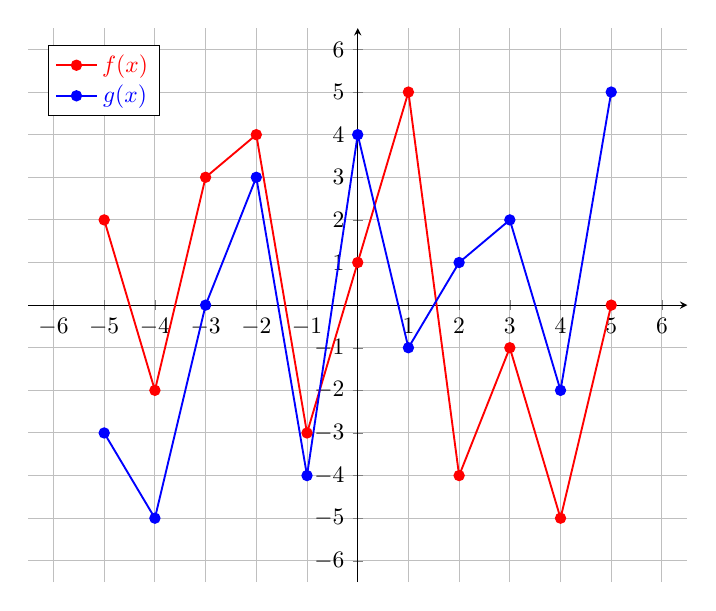
\begin{tikzpicture}[scale=0.85]
\begin{axis}
[xmin=-6.5, xmax=6.5, ymin=-6.5, ymax=6.5, xtick distance = 1, ytick distance = 1, axis lines=center, grid, width=4.5in, legend pos={north west}]
\addplot[color=red, mark=*, thick] coordinates {
(-5, 2) (-4,-2) (-3,3) (-2,4) (-1,-3) (0,1) (1,5) (2,-4) (3,-1) (4,-5) (5,0)
};
\addplot[color=blue, mark=*, thick] coordinates {
(-5, -3) (-4,-5) (-3,0) (-2,3) (-1,-4) (0,4) (1,-1) (2,1) (3,2) (4,-2) (5,5)
};
\addlegendentry{{\color{red}$f(x)$}};
\addlegendentry{{\color{blue}$g(x)$}};
\end{axis}
\end{tikzpicture}
\end{center}

\begin{multicols}{5}
\begin{enumerate}   \setcounter{enumi}{\value{Review}}  \setlength{\itemsep}{8pt}
    \item $(f + g)(2)$
    \item $(f - g)(1)$
    \item $(g - f)(-3)$
    \item $(fg)(4)$
    \item $\left(\frac{f}{g}\right)(0)$
\end{enumerate} \setcounter{Review}{\value{enumi}}
\end{multicols}

\newpage

Use the table below to find each.
\begin{center}
\begin{tabular}{c|c|c|c|c|c|c|c|c|c|c|c}

    $x$ & $-5$ & $-4$ & $-3$ & $-2$ & $-1$ & 0 & 1 & 2 & 3 & 4 & 5 \\ \hline 
    $f(x)$ & $-1$ & 3 & $-4$ & 5 & 0 & 4 & $-5$ & 2 & $-2$ & $-3$ & 1 \\ \hline 
    $g(x)$ & 4 & $-2$ & $-4$ & 1 & $-1$ & 3 & 0 & $-3$ & $-5$ & 2 & 5 \\
\end{tabular}
\end{center}
\begin{multicols}{5}
\begin{enumerate}	\setcounter{enumi}{\value{Review}}
\item $(f + g)(-1)$
\item $(f - g)(2)$
\item $(fg)(-3)$
\item $\left(\frac{f}{g}\right)(5)$
\item $(ff)(-4)$
\end{enumerate}	\setcounter{Review}{\value{enumi}}
\end{multicols}

\section{Operations with Functions: Domain}

Given $f(x)=\sqrt{2x+7}$ and $g(x) = 3x+3$, find the domain of each.
\begin{enumerate}
\item $(f + g)(x)$
\item $\left(\frac{f}{g}\right)(x)$
\item $\left(\frac{g}{f}\right)(x)$
\end{enumerate}


\section{Difference Quotient}

Write the difference quotient for each.
\begin{multicols}{3}
\begin{enumerate}
	\item $f(x) = 2x - 7$
	\item $g(x) = x^2 + 4x$
	\item $h(x) = -1$
\end{enumerate}	\setcounter{Review}{\value{enumi}}
\end{multicols}
\begin{multicols}{3}
\begin{enumerate}	\setcounter{enumi}{\value{Review}} 
	\item $f(x) = \frac{3}{x+2}$
	\item $g(x) = \sqrt{3x}$
	\item $f(x) = x^2 - 2x + 5$
\end{enumerate}	\setcounter{Review}{\value{enumi}}
\end{multicols}
\begin{multicols}{3}
\begin{enumerate}	\setcounter{enumi}{\value{Review}} 
	\item $g(x) = \frac{5}{x}$
	\item $f(x) = -2x^2 + 3x - 5$
	\item $g(x) = \frac{6}{2x+3}$
\end{enumerate}	\setcounter{Review}{\value{enumi}}
\end{multicols}
\begin{multicols}{3}
\begin{enumerate}	\setcounter{enumi}{\value{Review}} 
	\item $h(x) = \sqrt{7x+5}$
	\item $f(x) = -x^2 + x$
	\item $f(x) = 3x - 1$
\end{enumerate}	\setcounter{Review}{\value{enumi}}
\end{multicols}
\begin{multicols}{3}
\begin{enumerate}	\setcounter{enumi}{\value{Review}} 
	\item $f(x) = x^3 + 5x$
	\item $f(x) = \frac{6}{x+7}$
	\item $g(x) = \frac{9}{x}$
\end{enumerate}	\setcounter{Review}{\value{enumi}}
\end{multicols}
\begin{multicols}{3}
\begin{enumerate}	\setcounter{enumi}{\value{Review}} 
	\item $h(x) = \frac{5}{2x-1}$
\end{enumerate}	\setcounter{Review}{\value{enumi}}
\end{multicols}

\newpage


\section{Answer Key}

\section*{Adding, Subtracting, Multiplying, and Dividing Functions}

\begin{multicols}{2}
\begin{enumerate}
    \item $x^2-x-6$
    \item 38
    \item $x^2+x+4$
    \item $-1$
     \item $-3$
     \item $-4$
     \item $-2$
     \item $-6$
     \item $-3$
    \item 6
    \item $-3$
    \item 10
    \item $\frac{1}{4}$
    \item $-1$
    \item 5
    \item 16
    \item $\frac{1}{5}$
    \item 9
\end{enumerate}
\end{multicols}

\section*{Operations with Functions: Domain}
\begin{enumerate}
	\item $\left[-\frac{7}{2}, \infty\right)$
    \item $\left[-\frac{7}{2}, -1\right) \cup (-1, \infty)$
    \item $\left(-\frac{7}{2}, \infty\right)$
\end{enumerate}

\section*{Difference Quotient}
\begin{multicols}{3}
\begin{enumerate}
	\item 2
	\item $2x + h + 4$
	\item 0
\end{enumerate}	\setcounter{Review}{\value{enumi}}
\end{multicols}
\begin{multicols}{3}
\begin{enumerate}	\setcounter{enumi}{\value{Review}} 
    \item $\frac{-3}{(x+2)(x+h+2)}$
    \item $\frac{3}{\sqrt{3x+3h}+\sqrt{3x}}$
    \item $2x+h-2$
\end{enumerate}	\setcounter{Review}{\value{enumi}}
\end{multicols}
\begin{multicols}{3}
\begin{enumerate}	\setcounter{enumi}{\value{Review}} 
    \item $\frac{-5}{x(x+h)}$
    \item $-4x-2h+3$
    \item $\frac{-12}{(2x+3)(2x+2h+3)}$
\end{enumerate}	\setcounter{Review}{\value{enumi}}
\end{multicols}
\begin{multicols}{3}
\begin{enumerate}	\setcounter{enumi}{\value{Review}} 
    \item $\frac{7}{\sqrt{7x+7h+5}+\sqrt{7x+5}}$
    \item $-2x - h + 1$
    \item 3
\end{enumerate}	\setcounter{Review}{\value{enumi}}
\end{multicols}
\begin{multicols}{3}
\begin{enumerate}	\setcounter{enumi}{\value{Review}} 
    \item $3x^2 + 3xh + h^2 + 5$
    \item $\frac{-6}{(x+7)(x+h+7)}$
    \item $\frac{-9}{x(x+h)}$
\end{enumerate}	\setcounter{Review}{\value{enumi}}
\end{multicols}
\begin{multicols}{3}
\begin{enumerate}	\setcounter{enumi}{\value{Review}} 
    \item $\frac{-10}{(2x-1)(2x+2h-1)}$
\end{enumerate}
\end{multicols}